\documentclass{standalone}
\usepackage{tikz}
\usetikzlibrary{patterns}
\usetikzlibrary{positioning}
\usetikzlibrary{patterns, positioning}
\usetikzlibrary{shapes.misc}
\usepackage[outline]{contour}
\contourlength{1.5pt} 
\usepackage[sfdefault]{ClearSans}

\begin{document}
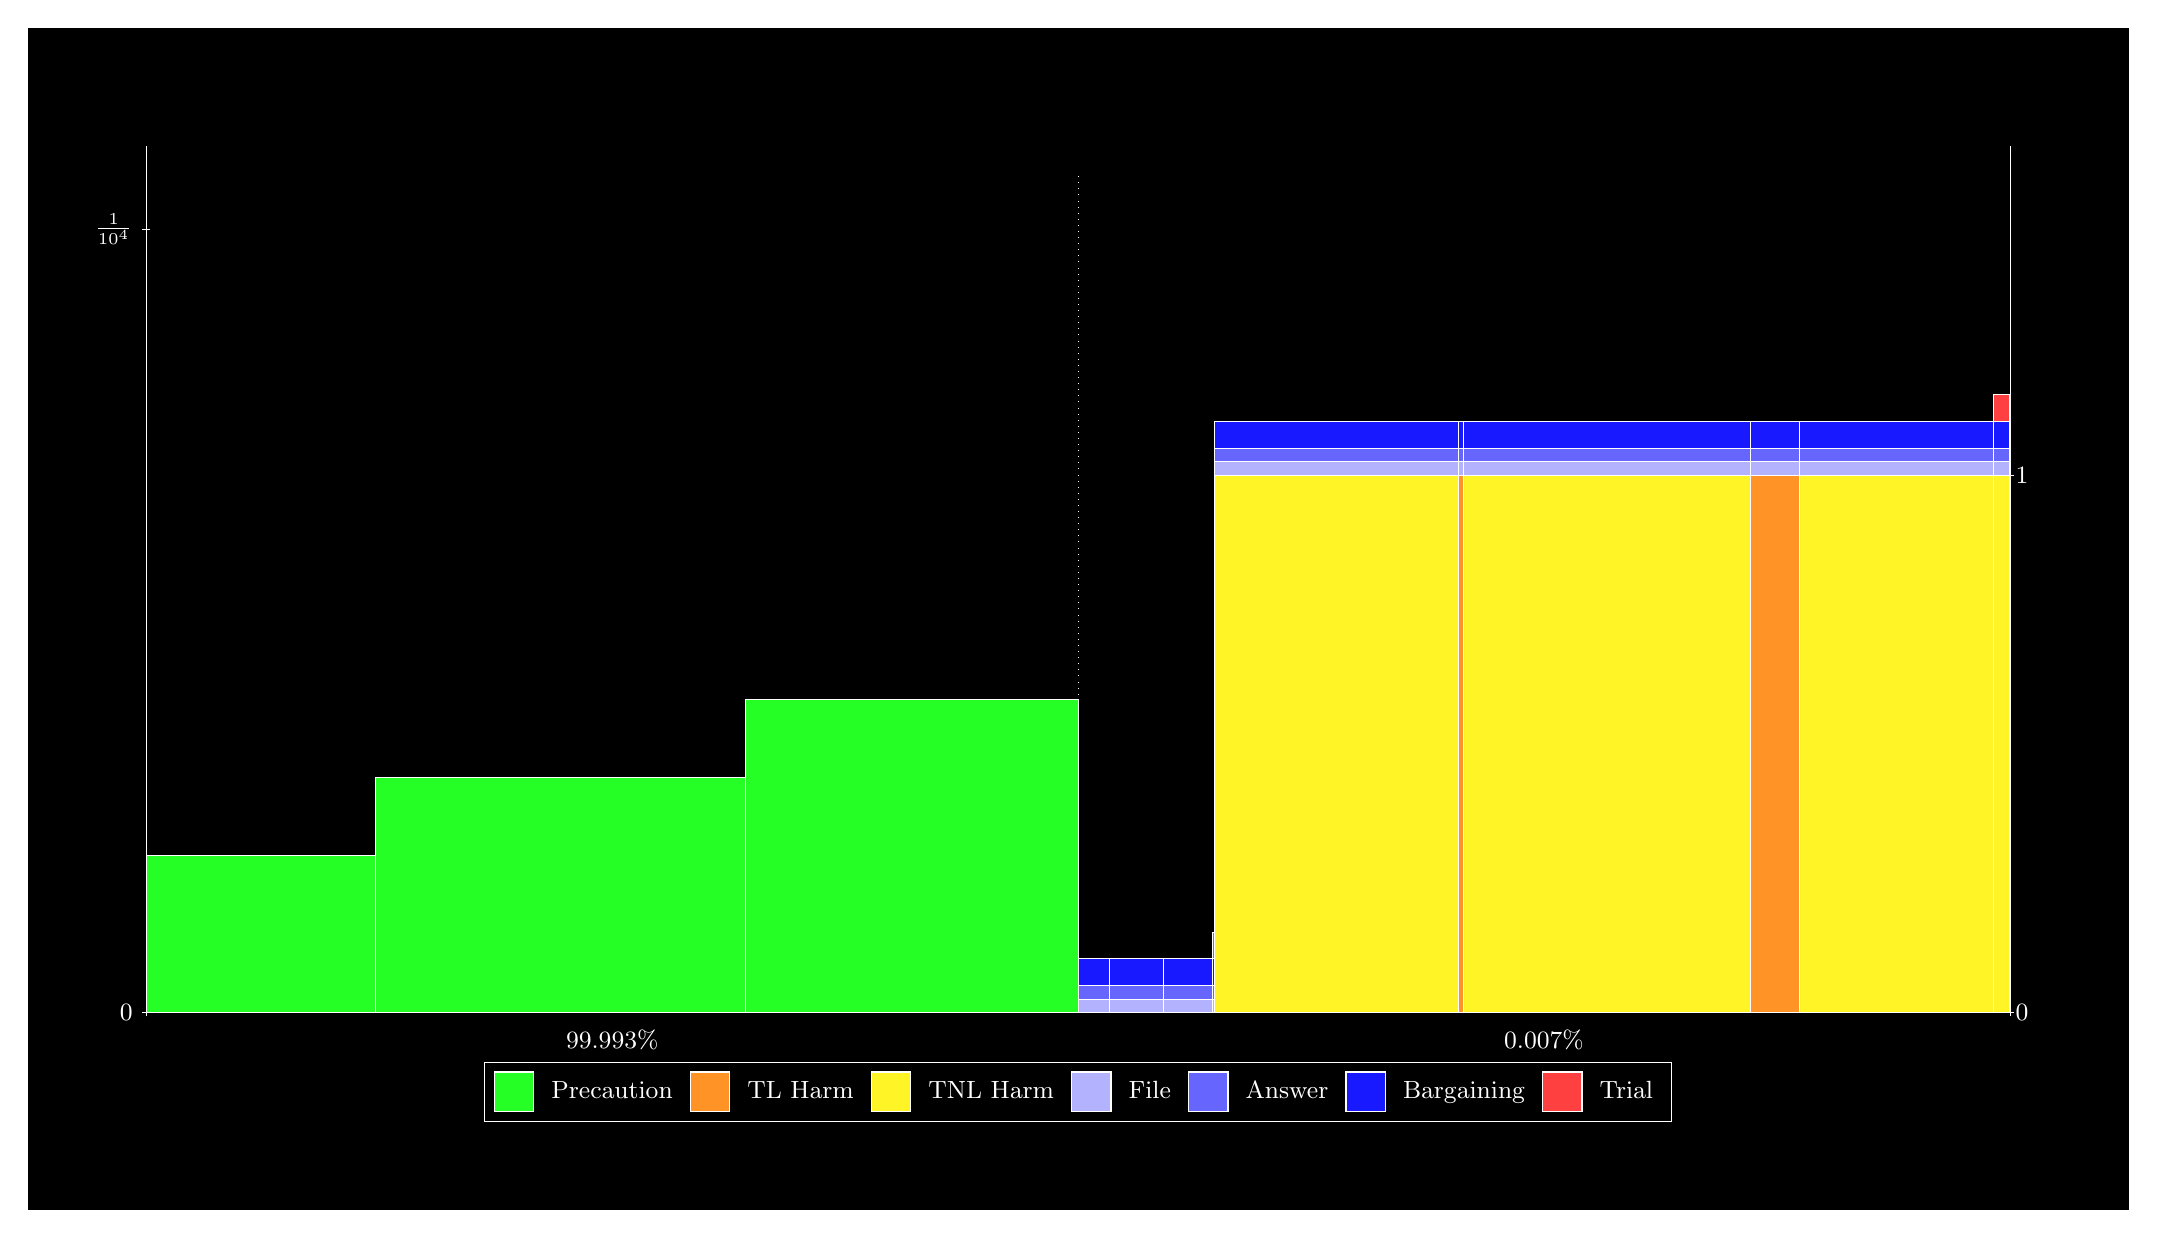
\begin{tikzpicture}
\draw[fill=black] (0,0) rectangle (26.667,15);
\draw[fill=green!85,draw=white,very thin] (1.5,2.5) rectangle (4.4122,4.4901);
\draw[fill=green!85,draw=white,very thin] (4.4122,2.5) rectangle (9.1125,5.4851);
\draw[fill=green!85,draw=white,very thin] (9.1125,2.5) rectangle (13.333,6.4801);
\draw[fill=green!85,draw=white,very thin] (13.333,2.5) rectangle (13.731,2.5001);
\draw[fill=blue!30,draw=white,very thin] (13.333,2.5001) rectangle (13.731,2.6707);
\draw[fill=blue!60,draw=white,very thin] (13.333,2.6707) rectangle (13.731,2.8414);
\draw[fill=blue!90,draw=white,very thin] (13.333,2.8414) rectangle (13.731,3.1826);
\draw[fill=green!85,draw=white,very thin] (13.731,2.5) rectangle (14.417,2.5002);
\draw[fill=blue!30,draw=white,very thin] (13.731,2.5002) rectangle (14.417,2.6708);
\draw[fill=blue!60,draw=white,very thin] (13.731,2.6708) rectangle (14.417,2.8414);
\draw[fill=blue!90,draw=white,very thin] (13.731,2.8414) rectangle (14.417,3.1826);
\draw[fill=green!85,draw=white,very thin] (14.417,2.5) rectangle (15.032,2.5003);
\draw[fill=blue!30,draw=white,very thin] (14.417,2.5003) rectangle (15.032,2.6709);
\draw[fill=blue!60,draw=white,very thin] (14.417,2.6709) rectangle (15.032,2.8415);
\draw[fill=blue!90,draw=white,very thin] (14.417,2.8415) rectangle (15.032,3.1827);
\draw[fill=green!85,draw=white,very thin] (15.032,2.5) rectangle (15.059,2.5001);
\draw[fill=blue!30,draw=white,very thin] (15.032,2.5001) rectangle (15.059,2.6707);
\draw[fill=blue!60,draw=white,very thin] (15.032,2.6707) rectangle (15.059,2.8414);
\draw[fill=blue!90,draw=white,very thin] (15.032,2.8414) rectangle (15.059,3.1826);
\draw[fill=red!75,draw=white,very thin] (15.032,3.1826) rectangle (15.059,3.5238);
\draw[fill=green!85,draw=white,very thin] (15.059,2.5) rectangle (18.163,2.5001);
\draw[fill=yellow!85,draw=white,very thin] (15.059,2.5001) rectangle (18.163,9.3245);
\draw[fill=blue!30,draw=white,very thin] (15.059,9.3245) rectangle (18.163,9.4951);
\draw[fill=blue!60,draw=white,very thin] (15.059,9.4951) rectangle (18.163,9.6657);
\draw[fill=blue!90,draw=white,very thin] (15.059,9.6657) rectangle (18.163,10.007);
\draw[fill=green!85,draw=white,very thin] (18.163,2.5) rectangle (18.223,2.5001);
\draw[fill=orange!85,draw=white,very thin] (18.163,2.5001) rectangle (18.223,9.3245);
\draw[fill=blue!30,draw=white,very thin] (18.163,9.3245) rectangle (18.223,9.4951);
\draw[fill=blue!60,draw=white,very thin] (18.163,9.4951) rectangle (18.223,9.6657);
\draw[fill=blue!90,draw=white,very thin] (18.163,9.6657) rectangle (18.223,10.007);
\draw[fill=green!85,draw=white,very thin] (18.223,2.5) rectangle (21.871,2.5002);
\draw[fill=yellow!85,draw=white,very thin] (18.223,2.5002) rectangle (21.871,9.3246);
\draw[fill=blue!30,draw=white,very thin] (18.223,9.3246) rectangle (21.871,9.4952);
\draw[fill=blue!60,draw=white,very thin] (18.223,9.4952) rectangle (21.871,9.6658);
\draw[fill=blue!90,draw=white,very thin] (18.223,9.6658) rectangle (21.871,10.007);
\draw[fill=green!85,draw=white,very thin] (21.871,2.5) rectangle (22.492,2.5002);
\draw[fill=orange!85,draw=white,very thin] (21.871,2.5002) rectangle (22.492,9.3246);
\draw[fill=blue!30,draw=white,very thin] (21.871,9.3246) rectangle (22.492,9.4952);
\draw[fill=blue!60,draw=white,very thin] (21.871,9.4952) rectangle (22.492,9.6658);
\draw[fill=blue!90,draw=white,very thin] (21.871,9.6658) rectangle (22.492,10.007);
\draw[fill=green!85,draw=white,very thin] (22.492,2.5) rectangle (24.96,2.5003);
\draw[fill=yellow!85,draw=white,very thin] (22.492,2.5003) rectangle (24.96,9.3246);
\draw[fill=blue!30,draw=white,very thin] (22.492,9.3246) rectangle (24.96,9.4953);
\draw[fill=blue!60,draw=white,very thin] (22.492,9.4953) rectangle (24.96,9.6659);
\draw[fill=blue!90,draw=white,very thin] (22.492,9.6659) rectangle (24.96,10.007);
\draw[fill=green!85,draw=white,very thin] (24.96,2.5) rectangle (25.154,2.5001);
\draw[fill=yellow!85,draw=white,very thin] (24.96,2.5001) rectangle (25.154,9.3245);
\draw[fill=blue!30,draw=white,very thin] (24.96,9.3245) rectangle (25.154,9.4951);
\draw[fill=blue!60,draw=white,very thin] (24.96,9.4951) rectangle (25.154,9.6657);
\draw[fill=blue!90,draw=white,very thin] (24.96,9.6657) rectangle (25.154,10.007);
\draw[fill=red!75,draw=white,very thin] (24.96,10.007) rectangle (25.154,10.348);
\draw[fill=green!85,draw=white,very thin] (25.154,2.5) rectangle (25.167,2.5001);
\draw[fill=orange!85,draw=white,very thin] (25.154,2.5001) rectangle (25.167,9.3245);
\draw[fill=blue!30,draw=white,very thin] (25.154,9.3245) rectangle (25.167,9.4951);
\draw[fill=blue!60,draw=white,very thin] (25.154,9.4951) rectangle (25.167,9.6657);
\draw[fill=blue!90,draw=white,very thin] (25.154,9.6657) rectangle (25.167,10.007);
\draw[fill=red!75,draw=white,very thin] (25.154,10.007) rectangle (25.167,10.348);
\draw[white,very thin] (1.5,2.5) -- (1.5,13.5);
\draw[white,very thin] (1.45,2.5) -- (1.55,2.5);
\node[font=\small,text=white, anchor=east] at (1.45, 2.5) {0};
\draw[white,very thin] (1.45,12.45) -- (1.55,12.45);
\node[font=\small,text=white, anchor=east] at (1.45, 12.45) {$\frac{1}{10^{4}}$};

\draw[white,dotted,very thin] (13.333,2.83) -- (13.333,13.17);
\draw[white,very thin] (25.167,2.5) -- (25.167,13.5);
\draw[white,very thin] (25.117,2.5) -- (25.217,2.5);
\node[font=\small,text=white, anchor=west] at (25.117, 2.5) {0};
\draw[white,very thin] (25.117,9.3244) -- (25.217,9.3244);
\node[font=\small,text=white, anchor=west] at (25.117, 9.3244) {1};

\draw[white,very thin] (1.5,2.5) -- (25.167,2.5);
\draw[white,very thin] (1.5,2.45) -- (1.5,2.55);
\node[font=\small,text=white, anchor=north] at (1.5, 2.45) {};
\draw[white,very thin] (25.167,2.45) -- (25.167,2.55);
\node[font=\small,text=white, anchor=north] at (25.167, 2.45) {};

\node[font=\small,text=white,anchor=south] at (7.4167, 1.9) {99.993\%};
\node[font=\small,text=white,anchor=south] at (19.25, 1.9) {0.007\%};
\draw (13.3333,2.5) node (B) {};
\begin{scope}[align=center]
\matrix[scale=0.5,draw=white,below=0.5cm of B,nodes={draw},column sep=0.1cm]{
\node[rectangle,draw,minimum width=0.5cm,minimum height=0.5cm,fill=green!85]{}; & \node[draw=none,font=\small,text=white]{Precaution}; &
\node[rectangle,draw,minimum width=0.5cm,minimum height=0.5cm,fill=orange!85]{}; & \node[draw=none,font=\small,text=white]{TL Harm}; &
\node[rectangle,draw,minimum width=0.5cm,minimum height=0.5cm,fill=yellow!85]{}; & \node[draw=none,font=\small,text=white]{TNL Harm}; &
\node[rectangle,draw,minimum width=0.5cm,minimum height=0.5cm,fill=blue!30]{}; & \node[draw=none,font=\small,text=white]{File}; &
\node[rectangle,draw,minimum width=0.5cm,minimum height=0.5cm,fill=blue!60]{}; & \node[draw=none,font=\small,text=white]{Answer}; &
\node[rectangle,draw,minimum width=0.5cm,minimum height=0.5cm,fill=blue!90]{}; & \node[draw=none,font=\small,text=white]{Bargaining}; &
\node[rectangle,draw,minimum width=0.5cm,minimum height=0.5cm,fill=red!75]{}; & \node[draw=none,font=\small,text=white]{Trial}; \\\\
};\end{scope}

\end{tikzpicture}
\end{document}